\section{Softvér}
\subsection{Arduino API}
\label{ArduinoLib}

Prvé vývojové prostredie, ktoré sme zvolili na programovanie arduina sa nazýva Arduino IDE\footnote[5]{Arduino Integrated Development Environment.} a využíva programovací jazyk C/C++ resp. jeho mutáciu, s pridanými špecializovanými príkazmi a funkciami. V rámci projektu AutomationShield existuje niekoľko rôznych Shieldov, ktoré však často využívajú rovnaké funkcie a príkazy. Z tohoto dôvodu bola vytvorená knižnica ,,AutomationShield'', ktorá v sebe zahŕňa niekoľko ďalších, často využívaných knižníc a súborov. Ide o funkcie potrebné pri riadení pomocou PID regulátora, vzorkovanie programu alebo mapovanie premenných. O jednotlivých funkciách, v rámci knižnice, si povieme viacej pri opise didaktických príkladov v Kap. \ref{Didaktické príklady}.

V rámci programovania knižníc využívame objektovo orientované programovanie \newline (OOP) \cite{oop}. Knižnice väčšinou rozdeľujeme na dva súbory. Prvým z nich je \verb|header| teda hlavička s koncovkou .h a druhý \verb|source| alebo zdrojový dokument s koncovkou .cpp. Header slúži ako akýsi navádzač a sklad pre premenné a funkcie, ktorý následne komunikuje so source dokumentom, v ktorom sú uložené samotné funkcie. Takéto rozdelenie súborov má za ciel zrýchlenie kompilácie programu \cite{546521}.


\subsubsection{Header}

Header súbor má niekoľko náležitostí, ktoré obsahuje. Na začiatok deklarujeme súbor samotný. Robíme to pomocou príkazu \verb|#define|. Avšak ak by sa takáto deklarácia nachádzala vo viacerých súboroch, a teda header súbor by sa definoval niekoľkokrát, spôsobovalo by to problém pri kompilácii kódu. Z toho dôvodu využívame príkazy \verb|#ifndef| spolu s \verb|#define|, ktoré zamedzujú násobnému definovaniu rovnakých súborov. 

Hneď za definovaním knižnice AeroShild.h môžeme do súboru vkladať ďalšie potrebné knižnice a to pomocou príkazu \verb|#include|. Následne určujeme premenné, ktoré môžu mať priradené fyzické čísla pinov na Arduine. 

\begin{lstlisting}[caption={Ukážka zdrojového kódu headeru.},captionpos=b]
#ifndef AEROSHIELD_H	 	 // Pokial nie je definovana AEROSHIELD_H
#define AEROSHIELD_H	 	 // Definuj kniznicu AEROSHIELD_H

#include "AutomationShield.h"    // Hlavna kniznica AutomationShieldu
#include <Wire.h>                // Kniznica potrebna pre komunikaciu I2C
#include <Arduino.h>		 // Zakladna arduino kniznica

#define AERO_RPIN A3             // Vstup z potenciometra
#define VOLTAGE_SENSOR_PIN A2    // Vstup pre meranie prudu 
#define AERO_UPIN 5              // Aktuator

----------------------Zdrojovy kod----------------------

#endif			   	 // Koniec if podmienky 
\end{lstlisting}



V časti \verb|Zdrojovy kod|, vytvárame \verb|triedu| (class), ktorá v sebe zahŕňa funkcie a premenné, ktoré sa nazývajú \verb|objekty| (objects). Trieda obsahuje podmnožinu objektov, ktoré vieme prepájať a spájať vo väčšie celky, vďaka čomu vieme dosiahnuť veľmi komplexné funkcie. Týmto funkciám a premenným vieme obmedziť prístup resp. ich dosah v rámci programu, pomocou modifikátorov prístupu (access modifiers). Tieto modifikátory delíme do štyroch skupín. Základný modifikátor je \verb|default|, teda akýsi predvolený prístup, ktorý nadobúdajú všetky funkcie a premenné automaticky. Ďalšími modifikátormi sú \verb|public|, teda funkcie a premenné verejne prístupné v triede aj mimo nej a modifikátor \verb|privat|, ktorý obmedzuje prístup len pre danú triedu. Posledným modifikátorom prístupu je \verb|protected|, čo je prístup chránený. V header súbore sa môže nachádzať jedna, alebo viacero tried, záleží to od logicky deliteľných úsekov kódu, alebo od preferencie programátora. 

Rozdelenie na public a privat má zmysel v prípade, ak chceme mať zadefinované premenné, pri ktorých nechceme aby sa dala externe zmeniť ich hodnota, alebo typ. V prípade privat takáto zmena nie je možná. Zmeniť takúto premennú môžeme len jej ručným prepísaním v zdrojovom súbore. V časti private deklarujeme funkcie, ktoré následne využívame v rámci triedy, alebo slúžia ako pomocné funkcie pri tvorbe komplexnejších častí kódu. V časti public sú funkcie viditeľné a schopné interagovať s inými triedami, ako aj s inými knižnicami. 


\subsubsection{Source}

Súbory \verb|header| a \verb|source| prepojíme príkazom \code{#include "AeroShield.h"}, ktorý vložíme na začiatok súboru. Ďalej v súbore deklarujeme jednotlivé funkcie, ktoré majú na začiatku zápisu, zvolený istý dátový typ. Dátové typy funkcií poznáme rôzne \cite{datovetypy}, najviac však v AeroShielde využívame typy \verb|void|, \verb|float| a \verb|bool|. 


\subsubsection{Popis použitých funkcií z knižnice AutomationShield}

Pri rôznych veľkostiach a rozsahoch číselných stupníc je dobré vyjadrovať hodnoty v percentách namiesto ich absolútnej hodnoty. Arduino ponúka funkciu \verb|map()|, ktorá však pracuje len s dátovým typom integer. Aby sme docielili vyššiu presnosť, potrebujeme mapovať dátový typ float. Na tento účel nám slúži funkcia \verb|mapFloat|. 

\begin{lstlisting}[caption={Zdrojový kód funkcie mapFloat.},captionpos=b]
float AutomationShieldClass::mapFloat(float x, float in_min, float in_max, float out_min, float out_max) 
{
return (x - in_min) * (out_max - out_min) / (in_max - in_min) + out_min; 
}
\end{lstlisting}


\subsubsection{Popis použitých funkcií z knižnice AeroShield}
\label{kodikSource}


Keďže na AeroShielde využívame senzor hall efektu, musíme s ním v prvom rade nadviazať komunikáciu a to pomocou sériovej komunikácie I$^{2}$C.

Táto komunikácia funguje na princípe master-slave. Master môže naraz komunikovať s viacerými zariadeniami a to na základe jedinečných adries zariadení, ktoré sa medzi sebou striedajú v komunikácii.

 Protokol I$^{2}$C využíva na odosielanie a prijímanie údajov dva vodiče resp. dve linky: 
\begin{itemize}
\item sériovú dátovú linku (SDA-serial data), cez ktorú sa posielajú údaje, 
\item sériovú hodinovú linku (SCL-serial clock), na ktorú arduino v pravidelných intervaloch posiela impulzy. 
\end{itemize}

Hodinový pin udáva tempo komunikácie a je ovládaný mastrom. Mení stav v pravidelných impulzoch z 0 (low), na 1 (high). Pri každej takejto zmene je na dátový pin poslaný jeden bit informácie. Tieto bity najskôr obsahujú adresu zariadenia slave, s ktorým chce master komunikovať, následne sa odosielajú bity príkazov. Keď sa táto informácia celá odošle, slave vykoná požiadavku a ak je to vyžadované, môže spätne mastrovi poslať údaje. Všetky tieto bity informácií sa posielajú na linke SDA \cite{idvac}.

   

\subsubsection{Funkcia readOneByte()}

 Funkcia \code{int AeroShield::readOneByte()}, získava 1 bajt informácii zo senzoru. Túto funkciu využívame napríklad na čítanie polohy kyvadla. 

\begin{lstlisting}[caption={Zdrojový kód funkcie readOneByte.},captionpos=b]
int AeroShield::readOneByte(int in_adr)         
{
	int retVal = -1;	 // Zadefinovanie pomocnej premennej
	Wire.beginTransmission(_ams5600_Address);// Zaciatok komunikacie 
	Wire.write(in_adr);	// Poziadavka na zaznamenianie uhlu kyvadla 
	Wire.endTransmission();	// Koniec komunikacie zo strany mastra
	Wire.requestFrom(_ams5600_Address, 1);	// Ziadost na odpoved  
	while (Wire.available() == 0);	// Cakaj pokial odpoved nepride  
	
	retVal = Wire.read();	// Zaznamenanie odpovede 
	
	return retVal;	// Zaslanie odpovede 
}
\end{lstlisting}

Ako môžeme vidieť v kóde funkcie, master najskôr osloví zariadenie slave, pomocou jeho adresy. Pri senzore \verb|AS5600| je adresa zariadenia v hexadecimálnej podobe 0x36. Následne zašle od výrobcu predprogramovanú žiadosť, ktorá zaznamená aktuálnu polohu magnetu resp. kyvadla. Následne je zaslaná požiadavka na odpoveď zo strany slave zariadenia, ktorá je zaznamenaná a odoslaná späť na miesto, z ktorého bola funkcia privolaná.

\subsubsection{Funkcia readTwoBytes()}

Funkcia \code{word AeroShield::readTwoBytes()} je podobná predošlej funkcii, s tým rozdielom, že získané su dva bajty informácií. Na konci funkcie ešte prebieha bitový posun\footnote[6]{Bitový posun je operácia vykonávaná so všetkými bitmi binárnej hodnoty, pri ktorej sa posúvajú o určený počet miest doľava alebo doprava \cite{biteShift}.}. 

\begin{lstlisting}[caption={Zdrojový kód funkcie readTwoBytes.},captionpos=b]
word AeroShield::readTwoBytes(int in_adr_hi, int in_adr_lo)        
{
	word retVal = -1;		// Zadefinovanie pomocnej premennej
	/* citanie "Low" bajtu */
	Wire.beginTransmission(_ams5600_Address);// Zaciatok komunikacie 
	Wire.write(in_adr);	// Poziadavka na zaznamenianie uhlu kyvadla 
	Wire.endTransmission();	// Koniec komunikacie zo strany mastra
	Wire.requestFrom(_ams5600_Address, 1);	// Ziadost na odpoved  
	while (Wire.available() == 0);	// Cakaj pokial odpoved nepride  

	int low = Wire.read();     	// Ulozenie prveho bajtu 
	/* citanie "High" bajtu */
	Wire.beginTransmission(_ams5600_Address);// Zaciatok komunikacie 
	Wire.write(in_adr);	// Poziadavka na zaznamenianie uhlu kyvadla 
	Wire.endTransmission();	// Koniec komunikacie zo strany mastra
	Wire.requestFrom(_ams5600_Address, 1);	// Ziadost na odpoved  
	while (Wire.available() == 0);	// Cakaj pokial odpoved nepride  
	
	word high = Wire.read();   	// Ulozenie druheho bajtu 
	
	high = high << 8;          	// Posun bitov
	retVal = high | low;
	
	return retVal;	   	  	// Zaslanie odpovede 
}
\end{lstlisting}

\subsubsection{Funkcia detectMagnet()}

Ďalšou dôležitou funkciou, je zistiť prítomnosť magnetu na kyvadle. Túto úlohu vykonáva funkcia \code{bool AeroShield::detectMagnet()}. Využívame ju vždy pri inicializácii AeroShieldu na to, aby sme zistili či nenastali problémy s magnetom, alebo so senzorom samotným. Na základe výstupu z funkcie vieme určiť či bol magnet detegovaný. Funkcia vráti na výstupe 1- pokiaľ sa magnet nachádza pri senzore a 0- pokiaľ magnet nie je zachytený. 

\begin{lstlisting}[caption={Zdrojový kód funkcie detectMagnet.},captionpos=b]
bool AeroShield::detectMagnet() 
{
	int magStatus;		// Pomocna premenna  
	int retVal = 0;		// Pomocna premenna
	magStatus = readOneByte(_stat);	// Prebieha komunikacia so senzorom                        
	
	if (magStatus & 0x20)		// Pokial je podmeinka splnena vrat 1, pokial nie je splnena vrat 0 
	retVal = 1;
	
	return retVal;			// Zaslanie odpovede 
}
\end{lstlisting}

\subsubsection{Funkcia getMagnetStrength()}

Pre správnosť fungovania hall senzoru je dôležité dodržať predpísanú vzdialenosť magnetu od senzoru. Výrobca udáva že najideálnejšia vzdialenosť je 0.5-3 mm, v závislosti na sile a veľkosti magnetu. Bolo by nepraktické túto vzdialenosť merať ručne. Použijeme preto funkciu \code{int AeroShield::getMagnetStrength()}. Môžeme si všimnúť, že táto funkcia používa rovnaký príkaz na komunikáciu so senzorom, ako aj funkcia \code{detectMagnet()} a to síce \verb|_stat|. Z toho vyplýva že \code{detectMagnet()} kontroluje nielen prítomnosť magnetu, ale aj jeho správnu vzdialenosť. Pokiaľ teda dostaneme z funkcie \code{detectMagnet()} ako výsledok 1, vieme že magnet je prítomný a zároveň v ideálnej vzdialenosti. Funkcia \code{getMagnetStrength()} je teda iba doplňujúcou funkciou, ktorá nám určí či sa magnet nachádza príliš blízko, alebo naopak veľmi ďaleko od senzoru. 

\begin{lstlisting}[caption={Zdrojový kód funkcie getMagnetStrength.},captionpos=b]
int AeroShield::getMagnetStrength()   
{
	int magStatus;                  // Pomocna premenna 
	int retVal = 0;                 // Pomocna premenna
	magStatus = readOneByte(_stat);	// Prebieha komunikacia so senzorom       
	
	if (detectMagnet() == 1)	// Pokial je splnena podmienka detectMagnet()
	{
		retVal = 2;  // Vrat 2, magnet je v idelnej vzdialenosti
		if (magStatus & 0x10)
		retVal = 1;  // Vrat 1, magnet je v prilis daleko
		else if (magStatus & 0x08)
		retVal = 3;  // Vrat 3, magnet je v prilis blizko
	}
	
	return retVal;                  // Zaslanie odpovede  
}
\end{lstlisting}

\subsubsection{Funkcia getRawAngle()}

Táto funkcia slúži na čítanie uhlu kyvadla. Výstupom tejto funkcie, je číslo s rozsahom 12 bitov, teda číslo od 0 do 4096, ktoré udáva momentálnu polohu kyvadla. 

\begin{lstlisting}[caption={Zdrojový kód funkcie getRawAngle.},captionpos=b]
word AeroShield::getRawAngle() 
{
	return readTwoBytes(_raw_ang_hi, _raw_ang_lo); // Prebieha komunikacia so senzorom, ktory rovno vrati vysledok pomocou prikazu return 
}
\end{lstlisting}

\subsubsection{Funkcia begin()}

Prvou z funkcií mimo komunikácie s rotačným enkóderom je \code{void AeroShield::begin(void)}, v ktorej sa ako prvé zapíše výstup z funkcie \code{detectMagnet()} ako premenná \verb|isDetected|. Funkcia \code{begin()} nastaví pin potrebný na ovládanie akčného člena, pomocou príkazu \verb|pinMode|, ako výstup (OUTPUT). Zároveň inicializuje sériovú komunikáciu I$^{2}$C. Príkaz na započatie komunikácie I$^{2}$C sa pri rôznych typoch dosiek, resp. architektúr mikroradiča Arduino líši. Použijeme preto podmienku \verb|#ifdef|, za ktorou nasleduje typ architektúry daného mikroradiča a príslušný príkaz pre začiatok sériovej komunikácie I$^{2}$C. V prípade Arduino UNO, je to príkaz \verb|Wire.begin()|. 

Zároveň je vo funkcii \code{begin()}, pomocou if podmienky, kontrolovaná premenná \verb|isDetected|. Pokiaľ bol magnet detegovaný, vypíše na sériový port správu ,,Magnet detected'' a while\footnote[7]{Cyklus while sa bude opakovať nepretržite, pokiaľ sa výraz vnútri zátvoriek () nestane nepravdivým.} cyklus, sa pomocou príkazu \verb|break| ukončí. Pokiaľ magnet detegovaný nebol, vypíše ,,Can not detect magnet'', no while cyklus pokračuje.  


\begin{lstlisting}[caption={Zdrojový kód funkcie begin.},captionpos=b]
void AeroClass::begin(void){                       
	bool isDetected = AeroShield.detectMagnet(); 
	// Detekcia magnetu 
	pinMode(AERO_UPIN,OUTPUT);	// Pin aktuatora
	
	#ifdef ARDUINO_ARCH_AVR		// Pre dosky s architekturov AVR
	Wire.begin();			// Pouzi objekt Wire
	#elif ARDUINO_ARCH_SAM      	// Pre dosky s architekturov SAM
	Wire1.begin();			// Pouzi objekt Wire1
	#elif ARDUINO_ARCH_SAMD     	// Pre dosky s architekturov SAMD
	Wire.begin();			// Pouzi objekt Wire
	#endif
	
	if(isDetected == 0 ){       	// Pokial magnet nie je detegovany
		while(1){               // While podmienka
		 if(isDetected == 1 ){	// Pokial sa magnet deteguje
		  AutomationShield.serialPrint("Magnet detected \n");	
		break;		    // Koniec while podmienky
		}
		else{               // Pokial magnet nie je detegovany
		  AutomationShield.serialPrint("Can not detect magnet \n");
			}
		}
	}       
} 
\end{lstlisting}

\subsubsection{Funkcia calibration()}

Funkcia \code{calibration()} slúži na prepočet a zaznamenanie nulovej polohy kyvadla, teda takej kedy je kyvadlo v rovnovážnej polohe. V ideálnom prípade by sa kyvadlo vždy po vypnutí motora vrátilo do rovnakej východzej polohy. Avšak kyvadlo je prepojené s motorom a shieldom pomocou káblov, ktoré tvoria odpor a teda kyvadlo sa vždy zastaví v inej nulovej polohe. 

Do funkcie vstupuje hodnota aktuálneho uhla kyvadla, z funkcie \code{getRawAngle()} ako premenná \verb|rawAngle|. Funkcia na začiatok vypíše text ,,Calibration running...'' a motorček zapneme na štvrť sekundy na výkon 20\%. Kyvadlo sa začne kývať a počkáme štyri sekundy, pokiaľ sa ustáli. Keď je kyvadlo ustálené zaznamenáme jeho hodnotu do premennej \verb|startAngle|. Následne prebieha for cyklus, ktorý zvukovo informuje o dokončenej kalibrácii pomocou troch pípnutí. 

\begin{lstlisting}[caption={Zdrojový kód funkcie calibration.},captionpos=b]
float AeroShield::calibration(word rawAngle) {  
	AutomationShield.serialPrint("Calibration running...\n");  
	startAngle=0;              // Vynulovanie premennej 
	analogWrite(AERO_UPIN,50); // Spustenie motora na vykon 20%
	delay(250);                // Cakaj 0.25s 
	analogWrite(AERO_UPIN,0);  // Vypnutie motora
	delay(4000);               // Cakaj 4s
	
	startAngle = rawAngle;     // Uloz hodnotu nuloveho uhla
	analogWrite(AERO_UPIN,0);  // Poistne vypnutie motora 
	for(int i=0;i<3;i++){      // Funkcia na zvukovu signalizaciu
		analogWrite(AERO_UPIN,1);     // Zapnutie motora
		delay(200);                   // Cakaj
		analogWrite(AERO_UPIN,0);     // Vypnutie motora
		delay(200);                   // Cakaj
	}
	
	AutomationShield.serialPrint("Calibration done");
	return startAngle;                    // Vrat hodnotu 
}
\end{lstlisting}

\subsubsection{Funkcia convertRawAngleToDegrees()}

Ako sme už spomínali v Kap. \ref{meruhl}, zaznamenávaná hodnota uhlu kyvadla je v rozmedzí od 0 do 4096 a tieto hodnoty sú priamo úmerné so stupňami od 0\textdegree  do 360\textdegree. 1\textdegree   predstavuje hodnotu približne 11.77 vo formáte raw. Funkcia teda prenásobí raw hodnotu číslom 0.087\textdegree, ktoré sme získali z Rov. \ref{RovnicaConvert} a predstavuje veľkosť rozlíšenia rotačného enkóderu. Výstupom funkcie je uhol kyvadla v stupňoch.
 \begin{align}
 	\label{RovnicaConvert}
 	  \dfrac{360^{\circ}}{4096} = 0.087^{\circ}
 \end{align}

\begin{lstlisting}[caption={Zdrojový kód funkcie convertRawAngleToDegrees.},captionpos=b]
float AeroShield::convertRawAngleToDegrees(word newAngle) {  
	float ang = newAngle * 0.087;    // 360/4096=0.087 x rawHodnota                             
	return ang;                      // Vrat hodnotu
}
\end{lstlisting}


\subsubsection{Funkcia referenceRead()}

Funkcia \code{referenceRead()} slúži na čítanie hodnoty z potenciometra, ktorý sa nachádza na shielde, a jeho následne premapovanie do percentuálnej podoby. Potenciometer využívame na manuálne ovládanie AeroShieldu a v ďalších funkciách, sa využíva hlavne jeho percentuálna hodnota. Vrátená hodnota je typu float, v rozsahu od 0.0\% do 100.0\%. 

\begin{lstlisting}[caption={Zdrojový kód funkcie referenceRead.},captionpos=b]
	  float AeroShield::referenceRead(void) {      
		referencePercent = AutomationShield.mapFloat(analogRead(AERO_RPIN), 0.0, 1024.0, 0.0, 100.0);  
		 // Premapovanie originalnej hodnoty 0.0-1023 na percentualny rozsah 0.0-100.0
		return referencePercent;      // Vrat percentualnu hodnotu 
	}
\end{lstlisting}
	
\subsubsection{Funkcia actuatorWrite()}	
	
Na ovládanie motora resp. jeho otáčok, používame funkciu \code{actuatorWrite()}. Do funkcie vstupuje percentuálna hodnota žiadaného výkonu motora. Táto hodnota je premapovaná na PWM signál, ktorý využívame na ovládanie motora. Tento signál následne vstupuje do ochrannej funkcie \code{constrainFloat()}, ktorá zabezpečí aby sa hodnota PWM signálu mohla pohybovať len v rozmedzí od 0.0 do 255.0. 
	
	
\begin{lstlisting}[caption={Zdrojový kód funkcie actuatorWrite.},captionpos=b]
	void AeroShield::actuatorWrite(float motorPercent) {   
		float mappedValue = AutomationShield.mapFloat(motorPercent, 0.0, 100.0, 0.0, 255.0);       
		// Vstupna percentualna hodnota 0.0-100.0 premapovana na hodnoty 0.0-255.0
		mappedValue = AutomationShield.constrainFloat(mappedValue, 0.0, 255.0);  
		// Bezpecnostna funkcia obmedzenia premapovanej hodnoty
		analogWrite(AERO_UPIN, (int)mappedValue);  // Zapisanie hodnoty na pin
	}
\end{lstlisting}
	
	
\subsubsection{Funkcia currentMeasure()}	
	
Poslednou funkciou AeroShieldu je \code{currentMeasure()}, ktorá slúži na zaznamenávanie prúdu, ktorý odoberá motor kyvadla. Pre presnejšie výsledky merania, využívame priemernú hodnotu prúdu, ktorú získavame pomocou for cyklu. 

Nepresnosť vzniká v dôsledku ovládania motora PWM signálom. Tým, že je motor prerušovane vypínaný a zapínaný, kolísa aj veľkosť odoberaného prúdu. 

Výsledná hodnota prúdu prechádza úpravami pomocou dvoch korekčných premenných, ktoré sme získali vďaka meraniam prúdu pomocou multimetra a následným porovnaním týchto hodnôt oproti hodnotám zo senzora. 

Prevod z napätia na prúd robíme podľa pokynov uvedených v zdrojovom dokumente senzoru. Pri tomto prevode využívame hodnotu shunt rezistora \verb|RS|, ako aj hodnotu rezistora \verb|RL|. 
  
	
\begin{lstlisting}[caption={Zdrojový kód funkcie currentMeasure.},captionpos=b]	
float AeroShield::currentMeasure(void){  
	for(int i=0 ; i<repeatTimes ; i++){     // For cyklus
	voltageValue= analogRead(VOLTAGE_SENSOR_PIN);     
	// Citanie hodnoty zo senzoru INA169 
	voltageValue= (voltageValue * voltageReference) / 1024;    
	// Mapovanie hodnoty zo senzoru, na realnu hodnotu napatia(referencne napatie je 5V)
	current= current + correction1-(voltageValue / (10 * ShuntRes));    
                // Vzorec na vypocet prudu
                // Is = (Vout x 1k) / (RS x RL)
}                                                                         	
	float currentMean= current/repeatTimes;   
	// Vypocet priemernej hodnoty  
	currentMean= currentMean-correction2;       // Korekcia
	if(currentMean < 0.000) currentMean= 0.0;                 
	                    // Korekcia nulovej hodnoty
	current= 0;         // Vynulovanie pomocnych premennych   
	voltageValue= 0;    // Vynulovanie pomocnych premennych   
	return currentMean; // Vrat hodnotu prudu v amperoch
}
\end{lstlisting}
	
\subsection{MATLAB}	
\label{matlabik}
	
V tomto programe, rovnako ako pri Arduino IDE, vieme príkazy a funkcie zapisovať do knižnice, odkiaľ si potom jednotlivé položky voláme do hlavného kódu. Z toho dôvodu bola zostavená knižnica \verb|AeroShield.m|. Knižnice v MATLABE môžu mať podobu súborov \verb|Header| a \verb|Source|, alebo funkcie zapíšeme len do jedného súboru s koncovkou \verb|.m|. 

V našom prípade ide o jeden súbor, na ktorého začiatku definujeme triedu súboru, pomocou príkazu \code{classdef AeroShield < handle ... end}. Za príkazom \verb|classdef| nasleduje názov našej triedy \verb|AeroShield| a porovnávací symbol $<$, za ktorým nasleduje ,,super trieda'' \verb|handle|. Super, alebo nad-trieda \verb|handle| je abstraktná trieda, ktorej inštancia sa nedá vytvoriť priamo. Táto trieda sa využíva na odvodenie iných tried, ktoré sú už konkrétnymi triedami, ktorých inštancie sú objektmi handle \cite{HANDLE}. 

Každá trieda môže následne obsahovať jeden alebo viacero triednych blokov. V knižnici AeroShield máme definované dva triedne bloky typu \verb|properties|. V prom bloku sa nachádzajú objekty pre dosku arduino a hall senzor. V druhom bloku definujeme všetky premenné, ktoré budeme ďalej v kóde využívať. Jedná sa hlavne o názvy a čísla pinov, ktoré používame na čítanie alebo zapisovanie hodnôt, ako aj o premenné, na výpočet prúdu odoberaného motorom. 

\begin{lstlisting}[caption={Knižnica AeroShield.m properties.},captionpos=b]
classdef AeroShield < handle

properties
	arduino;		% objekt dosky arduino 
	as5600;			% objekt hall senzoru
end

properties(Constant)
	AERO_UPIN = 'D5';          % pin aktuatora 
	AERO_RPIN = 'A3';          % pin potenciometra
	VOLTAGE_SENSOR_PIN = 'A2'; % pin na meranie prudu
	
	voltageReference = 5.0;    % referencne hodnota napatia 
	ShuntRes = 0.1;            % hodnota shunt rezitora v ohmoch
	correction1 = 4.1220;	   % korekcia  				  
	correction2 = 0.33;        % korekcia
	repeatTimes = 50;          % pocet cyklov pre vypocet priemernej hodnoty prudu 
end		
\end{lstlisting}
		
Nasleduje triedy blok \verb|methods|, v ktorom sú definované všetky funkcie. Keďže logika funkcií je rovnaká ako v Kap. \ref{kodikSource}, nebudeme si funkcie vysvetľovať po jednom. Na ukážku si opíšeme časť kódu \code{function begin(AeroShieldObject)}, v ktorej prebieha tvorba objektov pre arduino a hall senzor. Príkaz \verb|arduino()| slúži na vyhľadanie dosky arduino, pripojenej do počítača a nastavenie parametrov potrebných na komunikáciu s doskou. Rovnako sa odvolávame aj na objekt \verb|as5600|, ktorý vytvoríme pomocou príkazu \verb|device()|, v ktorom zadávame objekt dosky arduino, a adresu zariadenia I$^2$C. Poslednou funkciou je vypísanie správy a konfiguráciu pinu \verb|AERO_UPIN| ako výstup. 

\begin{lstlisting}[caption={Knižnica AeroShield.m properties.},captionpos=b]
function begin(AeroShieldObject)          % funkcia inicializacie
	AeroShieldObject.arduino = arduino(); % tvorba arduino objektu
	AeroShieldObject.as5600 = device(AeroShieldObject.arduino,'I2CAddress',0x36); % tvorba objektu sonzoru
	configurePin(AeroShieldObject.arduino,AeroShieldObject.AERO_UPIN, 'DigitalOutput') % konfiguracia pinu ako vystup
	disp('AeroShield initialized.') % vypis spravu
end
\end{lstlisting}

Zostávajúce funkcie, ako aj celý zdrojový kód knižnice \verb|AeroShield.m| sa nachádza v prílohe \ref{AeroShield.m}. 

\newpage
\subsection{Simulink}
\label{SimulinkLib}

Simulink, narozdiel od MATLABU alebo Arduino IDE, využíva grafické programátorské prostredie, ktoré je založené na prepájaní funkčných blokov, vyberaných z knižnice. Pre prácu s Arduinom, v rámci Simulinku, existuje knižnica \textit{Simulink Support Package for Arduino Hardware}, ako aj vytvorená knižnica AeroLibrary Obr. \ref{OBRAZOK 2.6.4}, ktorú využívame priamo pre funkcie AeroShieldu. V knižnici AeroLibrary sa nachádzajú tieto bloky: 
\begin{itemize}
	\item Reference read- čítanie referenčnej hodnoty, 
	\item Actuator write- ovládanie akčného členu, 
	\item Angle read- meranie výstupu, 
	\item AeroShield- súhrn blokov na zapisovanie akčného zásahu ako aj meranie regulovanej veličiny.
\end{itemize}
Jednotlivé bloky majú svoju vlastnú vnútornú štruktúru a nastavenia, ktoré sa dajú meniť priamo v bloku, alebo pomocou masky bloku. Maska je akési grafické okno, ktoré sa zobrazí po kliknutí na blok. Toto okno zobrazuje informácie o funkcionalite bloku, ako aj prvky, pomocou ktorých sa dá nastaviť vnútorná štruktúra bloku. Pre lepšiu orientáciu medzi blokmi, má každý priradený vlastný ilustračný obrázok. Bližšie si o tvorbe masky povieme v Kap. \ref{Maska}. 

\begin{figure}[!tbh]
	\centering
	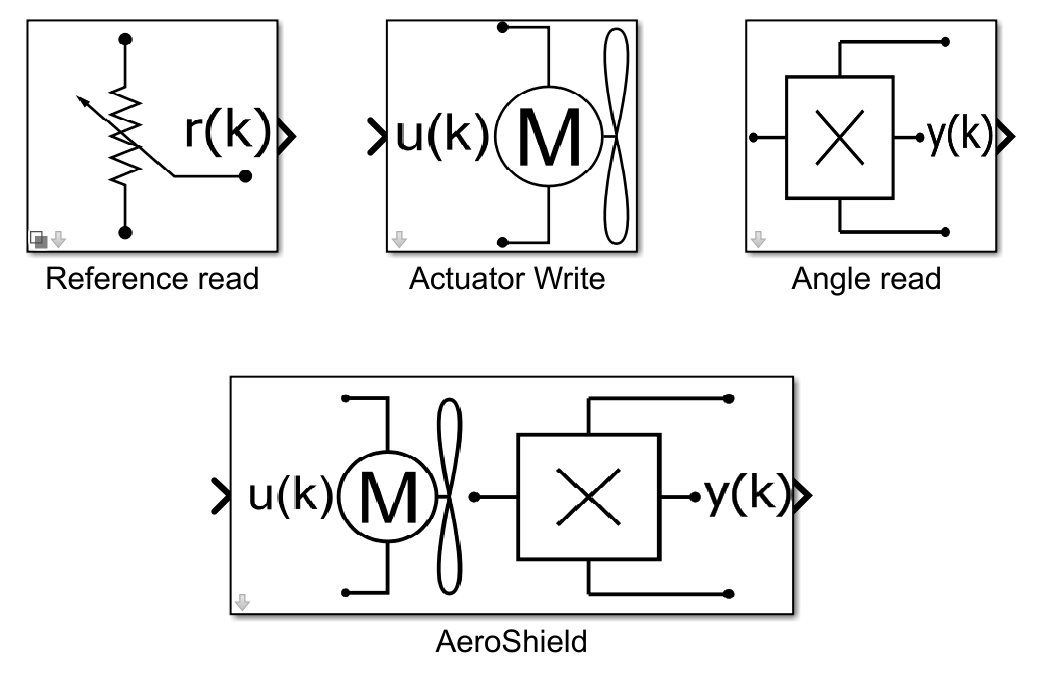
\includegraphics[width=125mm]{obr/AeroLib.png}
	\caption{Knižnica AeroLibrary.}\label{OBRAZOK 2.6.4}
\end{figure}

Blok \verb|Actuator Write| má najjednoduchšiu vnútornú štruktúru. Skladá sa z funkcie \verb*|Constrain|, ktorá prepočíta percentuálnu hodnotu vstupu na výstupný 8-bitový PWM signál. Tento signál posiela na Shield blok \verb*|PWM|, z knižnice \textit{Simulink Support Package for Arduino Hardware}. 

\subsubsection{Reference read}
\label{AngleRead}

V časti \verb|Reference read| máme na výber možnosť manuálnej, alebo automatickej trajektórie. Používateľ si z týchto možností vyberie pomocou tlačidiel v maske bloku. Vnútorná štruktúra sa ďalej skladá z troch podsystémov, z ktorých dva, pre manuálnu trajektóriu Obr. \ref{OBRAZOK 2.6.5}, sú takmer totožné. Rozdiel medzi nimi je taký, že pri použití niektorých druhov Arduina\footnote[8]{Due, MKR1000, MKR1010, MKRZero, Nano 33IoT.} je pri použitý bloku \verb|Analog input|, výstup v tvare 12-bitového čísla, narozdiel od 10-bitového, ako je tomu pri ostatných podporovaných modeloch Arduina. Načítaná hodnota je ďalej upravovaná do percentuálnej podoby, pomocou prenásobenia konštantou v bloku \verb*|gain|. 

Podsystém pre automatickú trajektóriu Obr. \ref{OBRAZOK 2.6.66} má viacero možností nastavenia. Ponúka možnosť zmeny pola referenčnej trajektórie, dĺžku trvania jednotlivých sekcií ako aj zmenu vzorkovacieho času. Viac informácií o bloku \verb|Reference read| nájdeme v Kap. \ref{Maska} na strane \pageref{Maska}. 

\begin{figure}[!tbh]
	\hfill
	\subfigure[Tri podsystémy bloku Reference read.]{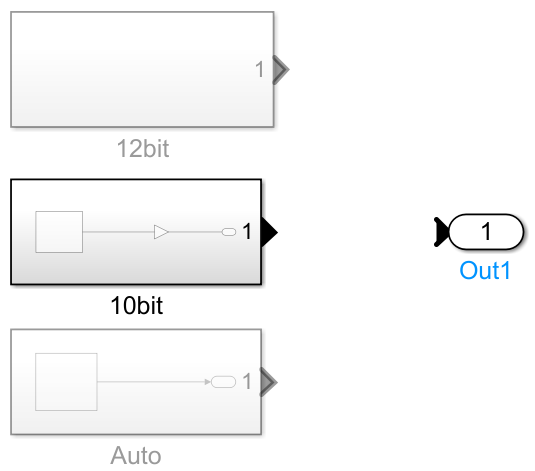
\includegraphics[width=6cm]{obr/Subsystem.png}}
	\hfill
	\subfigure[Podsystém pre 10-bitovú logiku.]{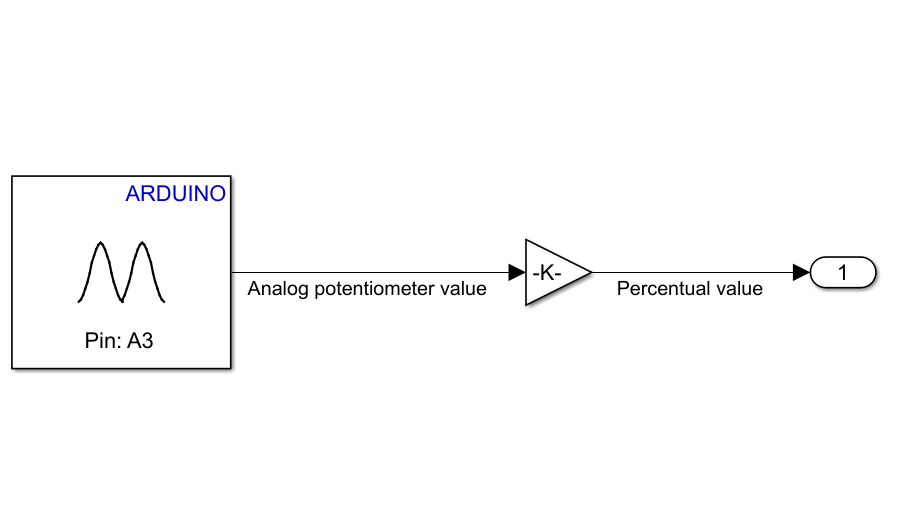
\includegraphics[width=9cm]{obr/10bit.png}}
	\hfill
	\caption{Reference read- Simulink.}\label{OBRAZOK 2.6.5}
\end{figure}

V \verb|MATLAB function| bloku, ktorý sa nachádza v podsystéme pre automatickú trajektóriu, nájdeme kód \ref{vrku}. Funguje na veľmi podobnom princípe ako v príklade \ref{matlabik}. Tento funkčný blok má 4 vstupy, z ktorých 3 zadávame v maske bloku, a 2 výstupy. Funkcia kontroluje čas, ako dlho sú spustené jednotlivé úseky automatickej trajektórie. Robí tak pomocou bloku \verb|Clock|, ktorý udáva aktuálny čas od spustenia simulácie. Pokiaľ je úsek trajektórie spustený dlhšie ako zadávame v maske bloku, funkcia automaticky prejde na ďalší úsek. Pokiaľ bola automatická trajektória ukončená, funkcia zastaví prebiehajúcu simuláciu. 



\begin{lstlisting}[caption={MATLAB function blok autiomatická trajektoria.},captionpos=b, label=vrku]
function [r, stopFlag] = fcn(clock, refVector, sectionLength, Ts)
persistent counter;
pauseTime = 2;

if isempty(counter)
counter = 1;
end
if clock > pauseTime
RefLength = length(refVector);
SectionDuration = sectionLength * Ts;
if (clock - pauseTime) <= (SectionDuration * counter)
r = refVector(counter);
stopFlag = 0;
else
counter = counter + 1;
if counter <= RefLength
r = refVector(counter);
stopFlag = 0;
else
r = refVector(counter-1);
stopFlag = 1; 
end
end
else
r = refVector(1);
stopFlag = 0;
end
end
\end{lstlisting}

\begin{figure}[!tbh]
	\centering
	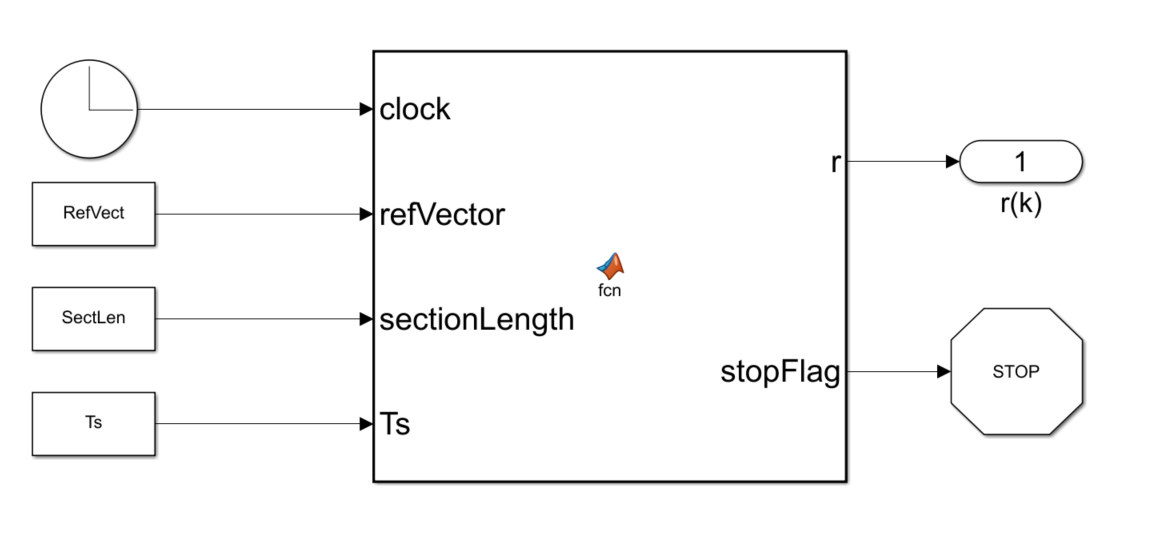
\includegraphics[width=100mm]{obr/AutoSimul.png}
	\caption{Automatická trajektória- Simulink.}\label{OBRAZOK 2.6.66}
\end{figure}

\subsubsection{Angle read}

Blok \verb|angle read| Obr. \ref{OBRAZOK 2.6.6} slúži na čítanie uhlu kyvadla, ako aj pre jeho bezpečnostnú kontrolu. Vnútorná štruktúra tohoto bloku sa dá rozdeliť na štyri menšie celky: 
\begin{itemize}
	\item zapisovanie príkazov na senzor,  
	\item čítanie uhlu kyvadla zo senzoru, 
	\item kalibrácia nulového uhlu kyvadla,
	\item kontrola uhlu kyvadla. 
\end{itemize}

\begin{figure}[!tbh]
	\centering
	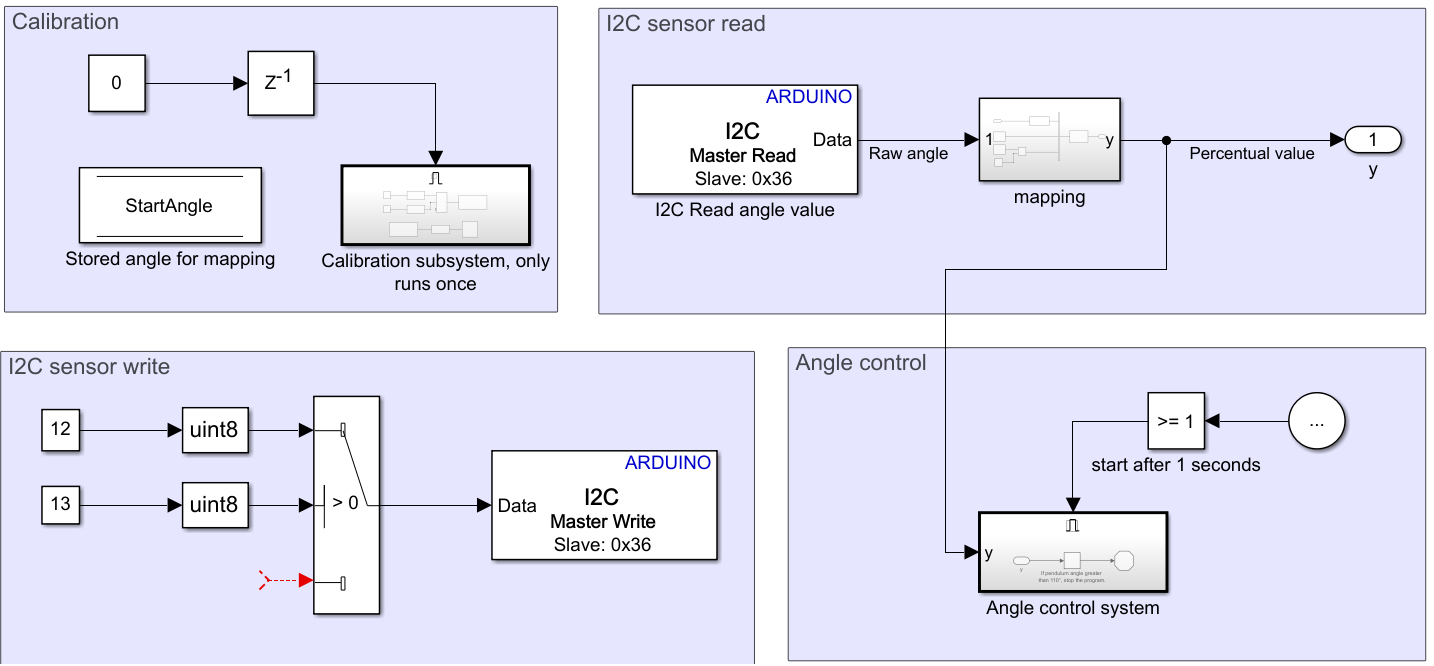
\includegraphics[width=\textwidth]{obr/AngleRead.png}
	\caption{Angle read- Simulink.}\label{OBRAZOK 2.6.6}
\end{figure}


\paragraph{I2C zápis}

Blok I2C Write Obr. \ref{OBRAZOK 2.6.6} (ľavý dolný roh), z knižnice \textit{Simulink Support Package for Arduino Hardware}, zapisuje na senzor striedavo hodnoty 12 a 13, ktoré slúžia ako príkaz pre čítanie a následné odoslanie hodnoty pootočenia kyvadla. Prepínanie medzi týmito dvomi hodnotami zabezpečuje automatický prepínač (Automatic switch). 

\paragraph{I2C čítanie}

Samotné čítanie uhlu zabezpečuje blok I2C Read Obr. \ref{OBRAZOK 2.6.6} (pravý horný roh), ktorého výstupom je 12-bitové číslo, predstavujúce aktuálne natočenie kyvadla. Tento výstup musíme previesť na uhlovú výchylku v rozmedzí od 0 do 360°. Tento prevod sa vykonáva v mapovacom podsystéme Obr. \ref{OBRAZOK 2.6.7}. Mapovanie funguje na rovnakom princípe ako v príklade \ref{MatlabPID}. Jednotlivé premenné vchádzajú do bloku \verb*|MUX|, ktorý slúži ako multiplexer\footnote[9]{Zariadenie, ktoré vyberá medzi viacerými analógovými alebo digitálnymi vstupnými signálmi a tieto preposiela na jednu výstupnú linku.}. Signál z multiplexoru vstupuje do \verb|fcn bloku|, ktorý prepája Simulink s MATLABOM. Zdrojový kód \ref{MAPfcn} zobrazuje funkciu vo vnútri tohoto bloku. 


\begin{figure}[!tbh]
	\centering
	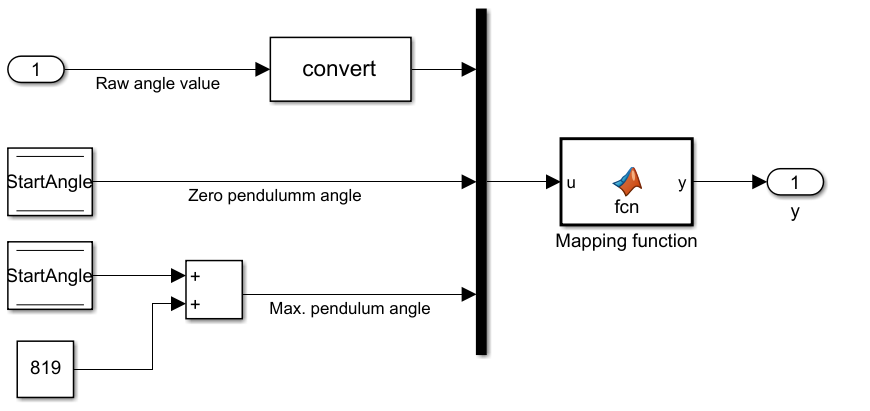
\includegraphics[width=\textwidth]{obr/SensMap.png}
	\caption{Mapovanie uhlu kyvadla- Simulink.}\label{OBRAZOK 2.6.7}
\end{figure}


\begin{lstlisting}[caption={Mapovacia funkcia vo fcn bloku.},captionpos=b,label=MAPfcn]
	function y = fcn(u)
	angMin=0;
	angMax=72;
	y = ((u(1) - u(2)) * (angMax - angMin)) /(u(3)- u(2)) + angMin ;
\end{lstlisting}


Proces získania premennej \verb|StartAngle|, ktorú využívame pri mapovaní, je opísaný v nasledujúcom odstavci. 

\paragraph{Kalibrácia} 
Kalibrácia prebieha vždy len raz a to pri spustení simulácie. V podsystéme (Enabled Subsystem) Obr. \ref{OBRAZOK 2.6.8}.a, ktorý je spustený len ak je do neho privedený signál, sa nachádzajú funkcie pre zapisovanie a čítanie informácii zo senzoru. Uhol ktorý je týmto podsystémom zaznamenaný pri spustený simulácie, sa uloží v bloku \verb|Data store Write|, ako premenná \verb|StartAngle| Obr. \ref{OBRAZOK 2.6.8}.b.                                                                                                                                                                                                                                                                                                                                                                                                                                                                                                                                                                                                                                                                                                                                                                                                                                                                                                                                                                                                                                                                                                                                                                                                                                                                                                                                                                                                                                                                                                                                                                                                                                                                                                                                                                                                                                                                                                                                                                                                                                                                                                                                                                                                                                                                                                                                                                                                                                                                                                                                                                                                                                                                                                                                                                                                                                                                                                                                                                                                                                                                                                                                                                                                                                                                                                                                                                                                                                                                                                                                                                                                                                                                                                                                                                                                                                                                                                                                                                                                                                                                                                                                                                                                                                                                                                                                                                                                                                                                                                                                                                                                                                                                                                                                                                                                                                                                                                                                                                                                                                                                                                                                                                                                                                                                                                                                                                                                                                                                                                                                                                                                                                                                                                                                                                                                                                                                                                                                                                                                                                                                                                                                                                                                                                                                                                                                                                                                                                                                                                                                                                                                                                                                                                                                                                                                                                                                                                                                                                                                                                                                                                                                                                                                                                                                                                                                                                                                                                                                                                                                                                                                                                                                                                                                                                                                                                                                                                                                                                                                                                                                                                                                                                                                                                                                                                                                                                                                                                                                                                                                                                                                                                                                                                                                                                                                                                                               

\begin{figure}[!tbh]
	\hfill
	\subfigure[Sústava pre zabezpečenie kalibrácie.]{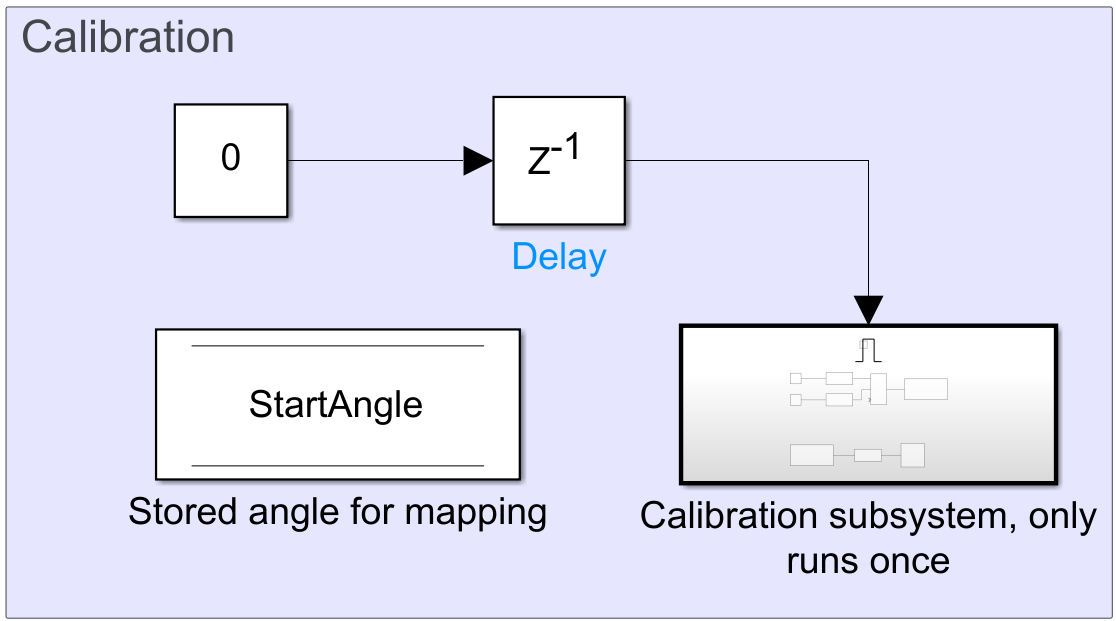
\includegraphics[width=6cm]{obr/Calibrat.png}}
	\hfill
	\subfigure[Podsystém pre zaznamenanie nulového uhla.]{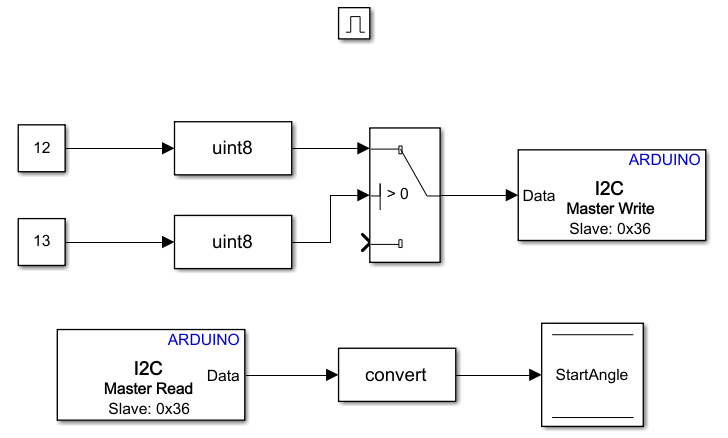
\includegraphics[width=9cm]{obr/calibDnu.png}}
	\hfill
	\caption{Kalibrácia- Simulink.}\label{OBRAZOK 2.6.8}
\end{figure}

\paragraph{Kontrola uhlu}

Kontrola uhlu kyvadla prebieha v podsystéme, ktorý je spustený jednu sekundu po spustení Obr. \ref{OBRAZOK 2.6.6} (pravý dolný roh). Časový posun je použitý z dôvodu občasného šumu premenných pri spustení príkladu. Tento šum môže spôsobiť nechcené výkyvy hodnoty uhlu kyvadla, ktoré by splnili podmienku v podsystéme a tým by zastavili priebeh simulácie. V podsystéme Obr. \ref{OBRAZOK 2.6.9}, sa nachádza blok \verb|Compare To Constant|, ktorý porovnáva hodnotu uhlu kyvadla, s daným maximálnym uhlom kyvadla. Táto hodnota je v našom prípade 110°. Pokiaľ kyvadlo dosiahne väčší uhol, ako je uhol dovolený, blok \verb|Stop Simulation| zastaví simuláciu.  

\begin{figure}[!tbh]
	\centering
	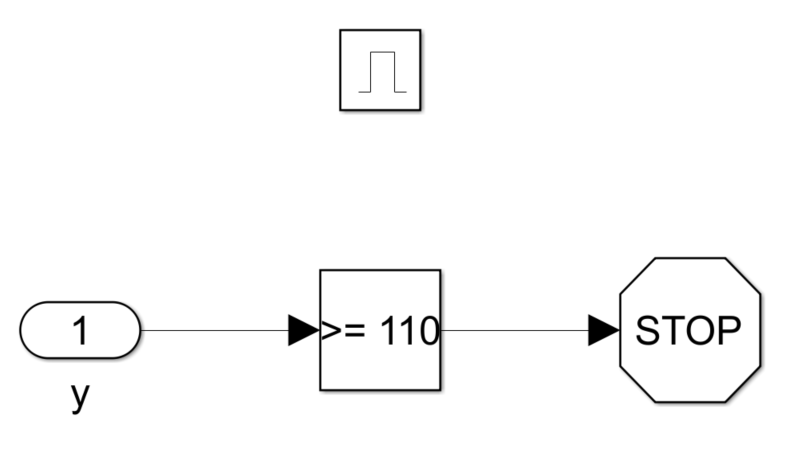
\includegraphics[width=100mm]{obr/AngleControl.png}
	\caption{Podsystém na kontrolu uhlu kyvadla.}\label{OBRAZOK 2.6.9}
\end{figure}

\newpage
\subsubsection{Tvorba masky}
\label{Maska}

Maska slúži ako vlastné používateľské rozhranie bloku resp. podsystému. Maskovaním bloku zapúzdrime blokovú schému tak, aby mala podla potreby, vlastné dialógové okná s nastaviteľnými parametrami, popisy bloku, výzvy na zadanie parametrov alebo texty s nápovedami. Vďaka maske je používanie a editácia blokov intuitívnejšia a vďaka textovým popisom funkcií jednoduchšia. Masku upravujeme pomocou editora, ktorý spustíme pravým kliknutím na blok, s následným výberom možnosti \verb|Mask|. V maske sa nachádzajú štyri hlavné editovacie rozhrania. 

Prvým z nich je záložka \verb|Icon & Ports|. V tomto okne upravujeme vzhľad bloku. Teda jeho zobrazenie, rotáciu, inicializáciu, alebo ikonu bloku. Pre všetky bloky v knižnici AeroLibrary, boli vytvorené vlastné ikony, ktoré sa do masky vkladajú príkazom \code{image('assets/Pote.png')}.

Ďalšou v poradí je záložka \verb|Parameters & Dialog|. V tejto sekcii nastavujeme vzhľad a funkcie masky, ktorá sa zobrazí po kliknutí na blok. V prípade bloku \verb|Reference read|, máme v maske na výber voľbu automatickej alebo manuálnej referenčnej trajektórie. Medzi týmito možnosťami si vyberáme pomocou tlačidiel (Radio button) Obr. \ref{OBRAZOK 2.6.100}, ktorých výber taktiež formátuje zobrazenie masky bloku. 

Pokiaľ si z tlačidiel vyberieme manuálnu trajektóriu, zobrazí sa ďalšia možnosť výberu, a tou je model dosky Arduino. Ide o roletové, alebo ,,popup'' menu, v ktorom si vyberieme typ dosky s ktorou používame AeroShield. Dôvod tohoto výberu je opísaný v Kap. \ref{AngleRead}, na strane \pageref{AngleRead}. Pokiaľ si zvolíme Automatickú referenčnú trajektóriu, možnosť voľby dosky sa nezobrazí. Namiesto toho sa zobrazia možnosti nastavenia automatickej trajektórie. Táto funkcia je vykonávaná automaticky, zdrojovým kódom \ref{Callback}, ktorý sa nachádza v časti \verb|Callback|, v nastaveniach tlačidiel voľby trajektórie. 

\begin{lstlisting}[caption={Callback funkcia.},captionpos=b,label=Callback]
ref = get_param(gcb,'ref');
if strcmp(ref(1),'M')
set_param(gcb,'MaskVisibilities',{'on';'on';'off';'off';'off';'off'}),
else
set_param(gcb,'MaskVisibilities',{'on';'off';'on';'on';'on';'on'}),
end
\end{lstlisting}

Pomocou príkazu \verb|get_param|, sa nám do premennej \verb|ref|, uloží výber tlačidla v maske. Príkaz \verb|gcb| vráti cestu
daného bloku v aktuálnom systéme. Podmienka \verb|if| kontroluje ktorú z možností sme si vybrali, pomocou príkazu \verb|strcmp|, ktorý porovnáva prvé písmeno z premennej \verb|ref|, s písmenom 'M' (Manual). Pokiaľ sa tieto zhodujú, príkaz \verb|set_param|, spolu s príkazom \verb|MaskVisibilities|, nastaví polia tlačidiel ako viditeľné, teda s hodnotou \verb|'on'|. Pokiaľ sa písmená nezhodujú a teda bola vybraná trajektória automatická, možnosť výberu dosky Arduino, je skrytá príkazom \verb|'off'| a namiesto nej, sa zobrazia ďalšie štyri editovateľné polia. 

\verb|Initialization| tvorí tretiu záložku v maske. V tejto záložke môžeme pridávať MATLAB kód, ktorý ovláda a formátuje podsystémy. V maske bloku \verb|Reference read |, máme v tejto záložke vložený kód \ref{Initialization}. Podľa pravdivosti \verb|if| podmienky, príkaz \newline \verb|set_param(gcb,'LabelModeActiveChoice'| aktivuje podsystém bloku, ktorého názov je uvedený ako tretí parameter v zátvorke príkazu. 

\begin{lstlisting}[caption={Initialization- maska Reference read.},captionpos=b,label=Initialization]
	ref = get_param(gcb,'ref');
	model = get_param(gcb,'model');
	if strcmp(ref,'Manual')
	if strcmp(model,'Due')
	set_param(gcb,'LabelModeActiveChoice', '12bit');
	elseif strcmp(model,'MKR1000')
	set_param(gcb,'LabelModeActiveChoice', '12bit');
	elseif strcmp(model,'MKR1010')
	set_param(gcb,'LabelModeActiveChoice', '12bit');
	elseif strcmp(model,'MKRZero')
	set_param(gcb,'LabelModeActiveChoice', '12bit');
	elseif strcmp(model,'Nano 33IoT')
	set_param(gcb,'LabelModeActiveChoice', '12bit');
	elseif strcmp(model,'Others') 
	set_param(gcb,'LabelModeActiveChoice', '10bit');
	end
	end
	if strcmp(ref,'Automatic')
	set_param(gcb,'LabelModeActiveChoice', 'Auto');
	end
\end{lstlisting}


\begin{figure}[!tbh]
	\centering
	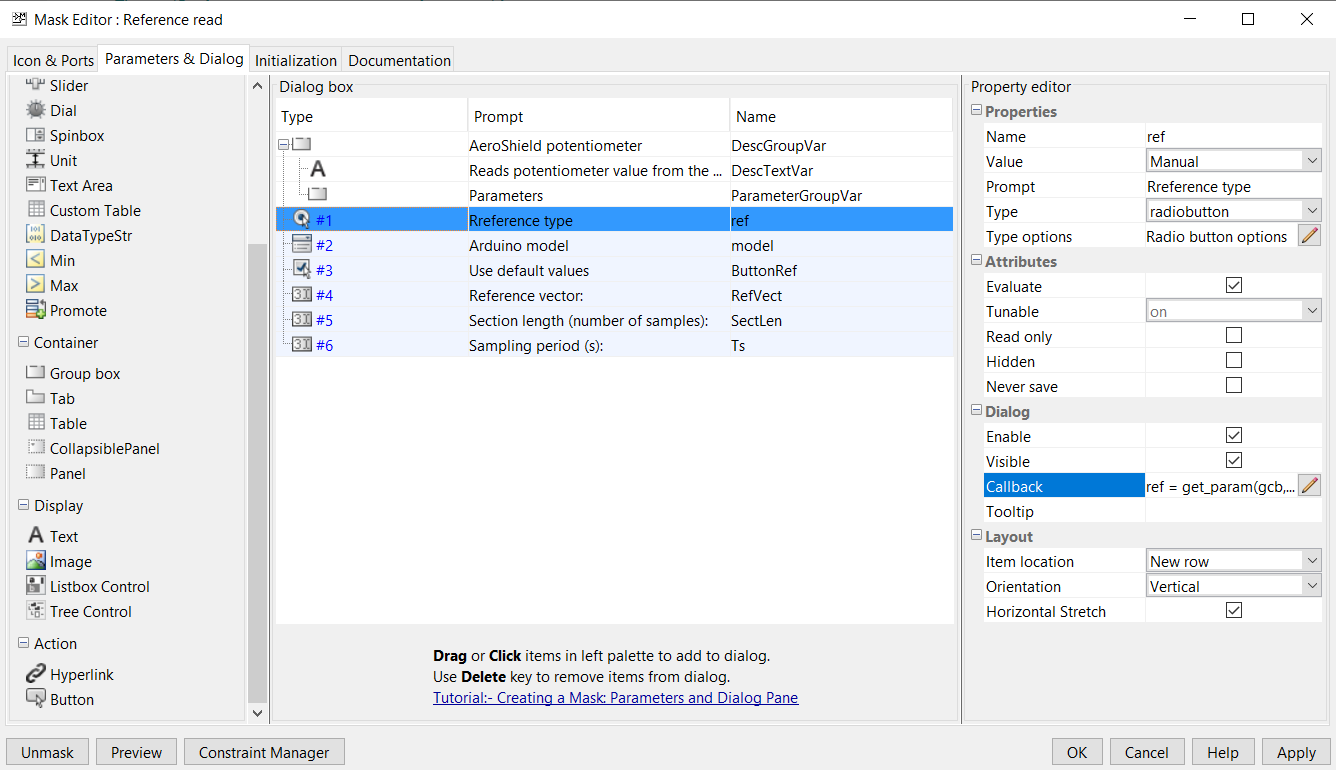
\includegraphics[width=\textwidth]{obr/ParamAnd.png}
	\caption{Nastavenia parametrov masky bloku Reference read.}\label{OBRAZOK 2.6.101}
\end{figure}


\begin{figure}[!tbh]
	\hfill
	\subfigure[Nastavenia masky pri výbere manuálnej trajektórie.]{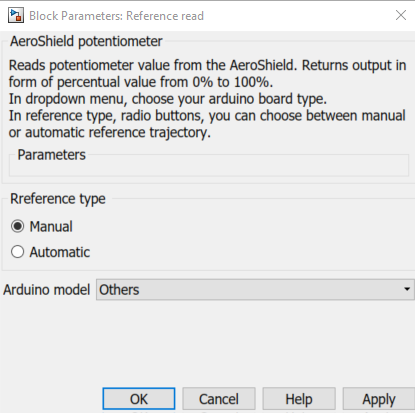
\includegraphics[width=7.3cm]{obr/Maska.png}}
	\hfill
	\subfigure[Zobrazenie masky pri výbere automatickej trajektórie.]{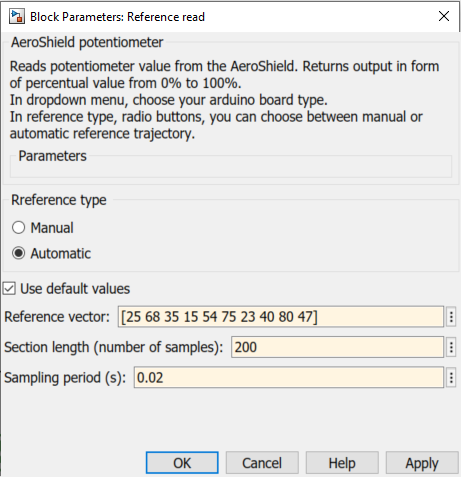
\includegraphics[width=7cm]{obr/MaskaA.png}}
	\hfill
	\caption{Reference read- Simulink.}\label{OBRAZOK 2.6.100}
\end{figure}

